\documentclass[11pt,a4paper]{article}

%% ---------------------------------------------------------------------------
%%  Encoding, fonts, layout
%% ---------------------------------------------------------------------------
\usepackage[T1]{fontenc}
\usepackage[utf8]{inputenc}
\usepackage{lmodern}
\usepackage{microtype}
\usepackage[margin=1in]{geometry}
\usepackage{setspace}
\usepackage{xurl} % Better URL breaking
\setlength{\emergencystretch}{3em} % Prevent overfull boxes in paragraphs

%% ---------------------------------------------------------------------------
%%  Math, theorems, symbols
%% ---------------------------------------------------------------------------
\usepackage{amsmath,amssymb,amsthm}
\usepackage{mathtools}

\newtheorem{theorem}{Theorem}[section]
\newtheorem{proposition}[theorem]{Proposition}
\theoremstyle{remark}
\newtheorem*{proofsketch}{Proof sketch}

%% ---------------------------------------------------------------------------
%%  Graphics, figures, tables
%% ---------------------------------------------------------------------------
\usepackage{graphicx}
\usepackage{booktabs}
\usepackage{array}
\usepackage{longtable}
\usepackage{caption}
\usepackage{tikz}
\usetikzlibrary{shapes,arrows.meta,positioning,calc}

%% ---------------------------------------------------------------------------
%%  Source listings (Equis / LLVM IR)
%% ---------------------------------------------------------------------------
\usepackage{xcolor}
\usepackage{listings}

\definecolor{lstbg}{gray}{0.97}
\definecolor{lstkw}{rgb}{0.00,0.30,0.55}
\definecolor{lstcm}{rgb}{0.30,0.50,0.30}
\definecolor{lststr}{rgb}{0.55,0.20,0.20}

\lstdefinelanguage{Equis}{
  morekeywords={Resource,Agent,Event,Commitment,roles,flow,in,out,from,to,
                fulfills,evaluated_by,execute,reverse,logic,fn,let,return,
                if,else,assert,sig,timestamp,reason,unit,decimals,id,status},
  sensitive=true,
  morecomment=[l]{//},
  morestring=[b]"
}

\lstset{
  basicstyle=\ttfamily\small,
  backgroundcolor=\color{lstbg},
  keywordstyle=\color{lstkw}\bfseries,
  commentstyle=\color{lstcm}\itshape,
  stringstyle=\color{lststr},
  showstringspaces=false,
  breaklines=true,
  breakatwhitespace=false,
  columns=flexible,
  frame=single,
  framerule=0pt,
  framesep=4pt,
  aboveskip=0.6em,
  belowskip=0.6em,
  xleftmargin=1em,
  xrightmargin=1em,
  literate={->}{{$\rightarrow$}}1
}

\lstnewenvironment{equiscode}{\lstset{language=Equis}}{}
\lstnewenvironment{llvmcode}{\lstset{language=LLVM,morekeywords={define,ret,call,add,sub,mul,sdiv,i64,void,entry}}}{}
\lstnewenvironment{plaincode}{\lstset{language={}}}{}

%% ---------------------------------------------------------------------------
%%  Bibliography (biblatex + biber, author-year style; natbib-compatible
%%  commands so \citet / \citep work as expected).
%% ---------------------------------------------------------------------------
\usepackage[backend=biber,
            style=authoryear,
            citestyle=authoryear-comp,
            natbib=true,
            maxcitenames=2,
            maxbibnames=99,
            uniquename=false,
            uniquelist=false,
            url=false,
            doi=true,
            isbn=false,
            sortlocale=en_US]{biblatex}
\addbibresource{equis.bib}

%% ---------------------------------------------------------------------------
%%  Hyperlinks (load late)
%% ---------------------------------------------------------------------------
\usepackage[hidelinks,
            pdftitle={Duality as a Type: Enforcing REA Accounting Semantics at Compile Time in the Equis Programming Language},
            pdfauthor={M Lintang Maulana Zulfan},
            pdfsubject={Programming languages; accounting type systems; REA},
            pdfkeywords={REA, accounting duality, type systems, fixed-point arithmetic, compiler verification, Equis}]{hyperref}
\usepackage{cleveref}

%% ---------------------------------------------------------------------------
%%  Title
%% ---------------------------------------------------------------------------
\title{Duality as a Type: Enforcing REA Accounting Semantics at Compile Time in the Equis Programming Language\thanks{DOI: \href{https://doi.org/10.5281/zenodo.20026585}{10.5281/zenodo.20026585}; Repository: \url{https://github.com/equis-lang/equis}}}

\author{M Lintang Maulana Zulfan\\
  Universitas Gadjah Mada, Indonesia\\
  \texttt{lintangmaulanazulfan@gmail.com}}

\date{\today}

%% ===========================================================================
\begin{document}
%% ===========================================================================

\maketitle

\begin{abstract}
Financial software sits at the center of modern economic infrastructure, yet
the programming languages used to build it provide no formal guarantees about
the semantic correctness of financial operations. Double-entry bookkeeping's
duality constraint, the rule that every economic event must produce balanced
inflows and outflows, is universally encoded at the application layer, where
it can be omitted, miscoded, or deliberately bypassed. No existing compiled
programming language includes a type rule for accounting duality.

This paper presents Equis, a compiled, self-hosting systems language that
elevates the Resource--Event--Agent (REA) model to first-class syntactic
constructs and enforces accounting duality as a static, compile-time
invariant. The compiler rejects any event declaration whose flow block is not
balanced before emitting a single instruction of LLVM~IR. Equis uses
fixed-point 64-bit integer arithmetic scaled by $10^{6}$ throughout,
eliminating IEEE 754 accumulation error from financial code paths entirely.
Memory management relies on automatic reference counting with a
resource-state borrow checker, giving deterministic, GC-pause-free behavior
in long-running settlement services. The compiler is self-hosted,
bootstrapped from ANSI~C, and verified via Diverse Double Compilation to
address Thompson's trusting-trust problem.

Contributions include the formal duality typing rule and its soundness
proof, the full REA primitive syntax integrated into a systems language,
role-based access control enforced statically at the agent-type level, an
append-only ledger primitive with compensating-transaction semantics, and a
20-module standard library covering collections, ledger management,
accounting, compliance, database access, HTTP, channels, and fibers. Equis
is, to the author's knowledge, the first compiled general-purpose language
to embed REA semantics in its type system. Compile-time duality enforcement
eliminates an entire class of financial logic errors with zero runtime
overhead.
\end{abstract}

\medskip
\noindent\textbf{Keywords:} REA model; accounting duality; type systems;
fixed-point arithmetic; compiler verification; financial software; Equis.

%% ---------------------------------------------------------------------------
\section{Introduction}\label{sec:intro}
%% ---------------------------------------------------------------------------

The correctness of financial software is not a niche concern. Accounting
systems process the transfers that underlie payroll, credit, settlement,
and taxation at civilizational scale. When such systems fail silently,
recording a debit without a corresponding credit, omitting a role check
from a transaction handler, or overwriting a ledger record rather than
reversing it, the consequences range from reporting fraud to systemic
financial instability. The Enron collapse illustrates how accounting
system failures at software and organizational layers interact to
produce outcomes that are catastrophic for public stakeholders
\citep{coffee_understanding_2002}.

The languages used to build financial software offer no protection
against this class of failure. C, C++, Go, Rust, and Python share no
understanding of what a financial transaction is. None of them knows
that the amount debited must equal the amount credited. None can reject,
at compile time, a function that writes to a debit account without a
matching credit. COBOL encodes accounting workflows procedurally, but it
does not formalize invariants; violations are runtime events, not
compile-time errors. The industry response has been to push correctness
into application frameworks, ORMs, and stored-procedure conventions, all
of which are bypassable by the programmer and invisible to the compiler.

\citet{mccarthy_rea_1982} established the REA (Resource--Event--Agent) model
as a generalized framework for accounting systems. REA identifies three
economic primitives present in every accounting domain: \emph{Resources}
are objects of economic value; \emph{Events} are occurrences that change
resource levels; \emph{Agents} are participants who control resources and
initiate events. \citet{geerts_ontological_2002} subsequently gave REA a
formal ontological grounding and \citet{geerts_policy-level_2006} extended it to
include policy-level authorization constraints. Over four decades, REA has
been applied to database schema design, business process modeling, and
markup languages. No prior work has lifted these primitives into a
compiled language's type system.

The thesis of this paper is straightforward. Accounting duality is not a
business rule to be enforced in application logic. It is a semantic
invariant that belongs in the language definition. Equis is an attempt
to close the gap between McCarthy's theoretical framework and the
languages that financial infrastructure is actually built with. The
central mechanism is simple: the compiler's type checker verifies, for
every \texttt{Event} declaration, that the sum of resource inflows
equals the sum of resource outflows in the same unit before emitting any
LLVM~IR. A program with an unbalanced event does not compile.

This paper makes several specific contributions to the formalization of
accounting systems. We introduce a systems language where REA
primitives---\texttt{Agent}, \texttt{Resource}, \texttt{Event}, and
\texttt{Commitment}---are implemented as reserved syntax keywords with
distinct semantic rules rather than user-space library abstractions. The
core theoretical contribution is a Gentzen-style duality typing rule,
complete with a structural induction proof of the Duality Theorem,
ensuring that any compiled program intrinsically preserves resource
totals across execution states. To eliminate IEEE 754 accumulation
errors in financial paths, the language enforces all \texttt{decimal}
values as fixed-point 64-bit integers scaled by $10^{6}$. We further
incorporate a resource-state borrow checker coupled with Automatic
Reference Counting (ARC) to provide deterministic memory reclamation and
enforce a strict use-after-move prevention mechanism. The language also
provides static Role-Based Access Control (RBAC) checked at compile
time, an immutable ledger primitive that supports only compensating
transactions without deletion, and a comprehensive standard library.
Finally, to address the problem of trusting trust, the compiler is
self-hosted, targets LLVM~IR, and is verified through Diverse Double
Compilation from an ANSI~C bootstrap.

\Cref{sec:motivation} motivates the design through concrete failure
modes in financial software. \Cref{sec:rea} reviews the REA model and
identifies the gap that Equis addresses. \Cref{sec:design} describes the
language design. \Cref{sec:impl} describes the compiler implementation.
\Cref{sec:semantics} presents the formal semantics. \Cref{sec:eval}
evaluates correctness and performance. \Cref{sec:related} surveys
related work. \Cref{sec:discussion} discusses limitations and future
directions.

%% ---------------------------------------------------------------------------
\section{Motivation: The Limits of Language in Financial Software}\label{sec:motivation}
%% ---------------------------------------------------------------------------

\subsection{The wrong abstraction level}

Modern financial applications enforce accounting correctness through a
combination of ORM conventions, database constraints, unit tests, and
code review. Each of these mechanisms operates below the language level:
the compiler that processes a debit function has no knowledge that a
corresponding credit function should exist, let alone that it should be
called with a matching amount before the transaction commits.
Correctness obligations fall entirely on individual programmers, and
programmer error is both inevitable and undetectable by tooling.

This structural arrangement is not a temporary limitation of current
compilers; it reflects a deliberate separation between general-purpose
programming languages and domain semantics. The same separation is
acceptable in domains where errors are recoverable or cheap. In
financial software, it is not. A transaction that credits without
debiting corrupts the ledger. A role check that is never called
authorizes unauthorized operations. An audit log that is overwritten
destroys the historical record. None of these errors produces a type
error in any mainstream language.

\subsection{Floating-point accumulation}

The IEEE 754 standard for floating-point arithmetic is the default
numeric representation in most programming languages. In the binary
floating-point model, many decimal fractions have no exact
representation: \texttt{0.1 + 0.2} does not equal \texttt{0.3}
\citep{goldberg_what_1991}. In isolation, the error is on the order of
$10^{-16}$; across millions of transactions, accumulated rounding
differences produce ledger imbalances that are real, persistent, and
difficult to trace. Financial institutions that use double-precision
floating-point for monetary computations spend engineering effort on
reconciliation procedures that exist solely to compensate for arithmetic
that is unreliable by design.

The standard industry remediation is to use a fixed-point or decimal
numeric type and to enforce its use through code review conventions.
This works until it does not. A programmer who accidentally computes an
intermediate result in \texttt{float} before converting to
\texttt{Decimal} introduces rounding without any compiler warning. The
language cannot distinguish a monetary amount from any other
floating-point number.

\subsection{Duality bypass and silent corruption}

Double-entry bookkeeping's duality constraint, requiring for every debit
a corresponding credit of equal amount, is the oldest formal invariant
in accounting, codified by Pacioli in 1494. In software, this constraint
is checked, when it is checked at all, by application-level validation
logic. The compiler does not participate. A function that writes a debit
record without writing a corresponding credit is syntactically and
type-theoretically correct in every existing general-purpose language.
The error manifests only when a subsequent audit or reconciliation
process detects the imbalance, often long after the fact.

A related failure mode is partial execution: a multi-step transaction
that succeeds on the debit step but fails on the credit step due to a
network or concurrency error leaves the ledger in an inconsistent state.
Database transactions address this at the persistence layer, but the
accounting constraint is not the same as ACID atomicity. A transaction
can be atomic and still violate duality if the application code is wrong
about which amounts to record.

\subsection{Privilege escalation via missing role checks}

Authorization checks in financial applications are typically implemented
as conditional branches: if the current user does not have the required
role, throw an exception. This pattern is correct when the branch
exists. When a programmer adds a new transaction handler and forgets the
role check, the function is callable by anyone with access to the
endpoint, and the compiler emits no warning. \citet{geerts_policy-level_2006}
established that authorization is a formal part of the REA ontology, but
their policy-level framework has never been implemented in a type
system.

\subsection{Audit trail mutability}

Financial regulations in most jurisdictions require an immutable audit
trail: every transaction must be recorded, and the record must not be
modifiable after the fact. The technical implementation of this
requirement in general-purpose languages is, again, a matter of
convention. Nothing prevents a programmer from issuing an
\texttt{UPDATE} or \texttt{DELETE} against a transaction table. The
constraint exists in the application logic or, at best, in database
row-level security policies, neither of which is visible to or enforced
by the programming language.

\subsection{Existing financial DSLs are not systems languages}

Several domain-specific languages address aspects of financial
correctness. \citet{andersen_compositional_2006} developed a compositional
specification language for commercial contracts with a formal
denotational semantics; \citet{henglein_formally_2020} extended this with
static analysis and formal verification. Marlowe, developed by IOHK, is a
financial contract DSL embedded in the Cardano blockchain. XBRL is a
markup language for financial reporting. None of these is a compiled
systems language for building financial infrastructure. They address
contract specification or regulatory reporting, not the general task of
writing servers, clearing pipelines, or accounting engines.

The distinction between a library and a language is the distinction
between a convention and an invariant. A library that implements REA
patterns establishes a convention that the programmer may follow; a
language whose syntax is REA cannot be compiled without following it.
Equis is the latter.

%% ---------------------------------------------------------------------------
\section{The REA Model and the Duality Constraint}\label{sec:rea}
%% ---------------------------------------------------------------------------

\begin{figure}[ht]
\centering
\resizebox{0.85\textwidth}{!}{
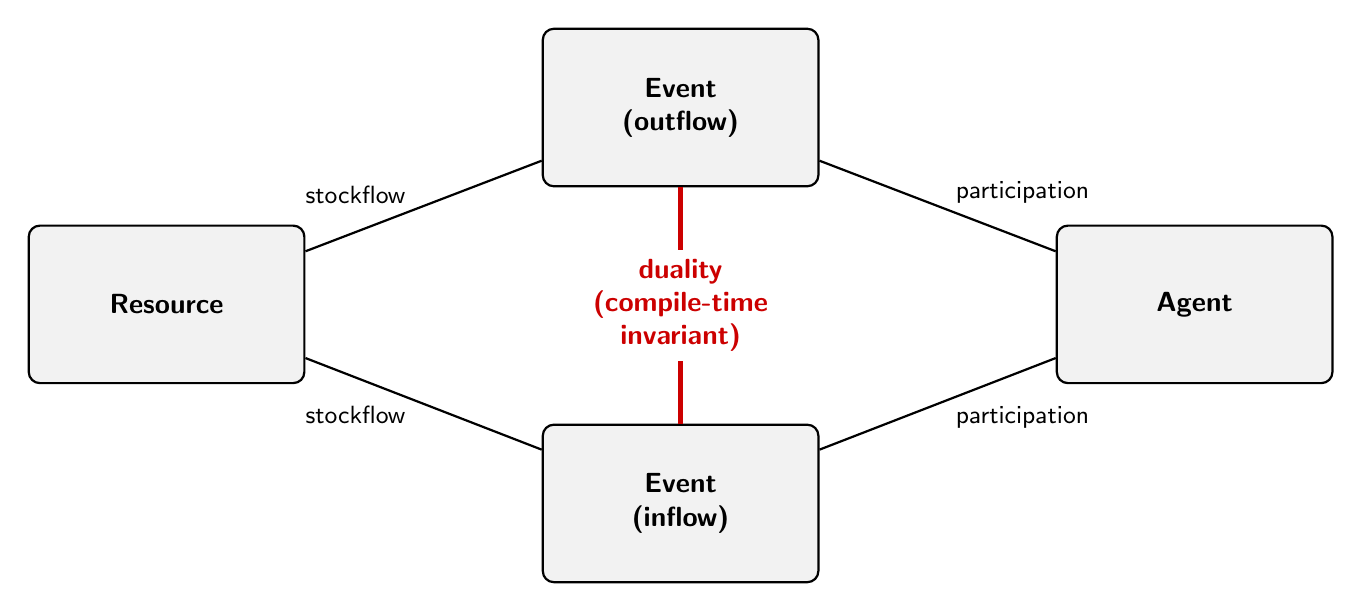
\begin{tikzpicture}[
  node distance=3cm and 3cm,
  box/.style={draw, thick, fill=gray!10, rounded corners,
              minimum width=3.5cm, minimum height=2cm, align=center,
              font=\sffamily\bfseries},
  duality/.style={draw, ultra thick, red!80!black}
]
\node[box] (outflow) {Event \\ (outflow)};
\node[box, below=3cm of outflow] (inflow) {Event \\ (inflow)};
\node[box, left=3cm of outflow, yshift=-2.5cm] (resource) {Resource};
\node[box, right=3cm of outflow, yshift=-2.5cm] (agent) {Agent};

\draw[thick] (outflow) -- (resource)
  node[midway, above left=-1mm and 1mm, font=\sffamily\small] {stockflow};
\draw[thick] (inflow)  -- (resource)
  node[midway, below left=-1mm and 1mm, font=\sffamily\small] {stockflow};
\draw[thick] (outflow) -- (agent)
  node[midway, above right=-1mm and 1mm, font=\sffamily\small] {participation};
\draw[thick] (inflow)  -- (agent)
  node[midway, below right=-1mm and 1mm, font=\sffamily\small] {participation};

\draw[duality] (outflow) -- (inflow)
  node[midway, fill=white, text=red!80!black, font=\sffamily\bfseries,
       align=center] {duality\\(compile-time\\invariant)};
\end{tikzpicture}
}
\caption{The three REA primitives and the relations that connect them.
The duality edge, highlighted, is the invariant that Equis lifts from a
modeling convention into a compile-time typing rule.}
\label{fig:rea}
\end{figure}

\subsection{Resources, events, and agents}

\citet{mccarthy_rea_1982} identified three primitives that appear in every
accounting domain, regardless of the specific chart of accounts or
industry context. A \textbf{Resource} is an economic object of value
that is controlled by an agent, such as inventory, cash, equipment, or
intellectual property. An \textbf{Event} is an occurrence that changes
the level of one or more resources, such as a sale, a payment, or a
shipment. An \textbf{Agent} is an individual or organization that
participates in events, either by initiating them or by being the source
or destination of resource transfers.

Every accounting entry in this model is, at bottom, an event that moves
a resource from one agent to another. The duality axiom follows
directly: if a resource leaves one agent, it must arrive at another. The
sum of outflows equals the sum of inflows. This is McCarthy's
generalization of Pacioli's double-entry principle, freed from the
specific categories of debit and credit.

\subsection{Ontological grounding}

\citet{geerts_ontological_1999,geerts_ontological_2002} gave REA a formal
ontological grounding using description logic and first-order
predicates. Resources, Events, and Agents are not merely data
categories; they are defined by their relationships. The
\emph{stockflow} relationship connects events to resources. The
\emph{duality} relationship connects paired events (a transfer and its
reciprocal). The \emph{participation} relationship connects events to
agents with specific roles.

The 2002 paper explicitly formalized the duality axiom as a logical
constraint: for every economic event, there must exist a paired event of
the opposite type (increment and decrement) involving the same resource.
This constraint is a theorem in the REA ontology, not merely a
convention.

\subsection{Policy-level extensions}

\citet{geerts_policy-level_2006} extended REA to include authorization
policies: which agents, in which roles, may initiate which events.
These policy specifications are part of the REA enterprise information
architecture, not an add-on. The formal model includes role definitions,
commitment structures that record obligations before execution, and
execution guards that verify role compatibility at runtime.

Equis implements both the structural REA constraints (duality,
stockflow) and the policy-level constraints (RBAC) at the language
level. The 2006 framework is, in Equis, not a modeling artifact but
executable code whose correctness is verified by the compiler.

\subsection{Closest prior work: the REA-DSL}

The closest prior work is the REA-DSL by \citet{sonnenberg_rea-dsl_2011}, a
domain-specific modeling language for business models based on the REA
ontology. The REA-DSL provides a graphical and textual notation for
specifying REA models and supports model validation against the
ontological constraints. It is, however, a modeling language, not a
compiled programming language. It produces models that describe
accounting structures; it does not produce machine code that runs
financial operations. Duality is validated in the modeling tool, not
enforced by a compiler.

\subsection{The gap}

All existing uses of REA, including database schema design, ontology
engineering, markup languages, and modeling tools, operate at a layer
above the compiler. No prior work enforces REA invariants at compile
time in a general-purpose systems language. The programs that actually
run financial infrastructure, the ones that write to databases, process
HTTP requests, and manage in-memory state, are written in languages that
are entirely ignorant of the accounting structure they implement. Equis
addresses this gap.

%% ---------------------------------------------------------------------------
\section{Language Design}\label{sec:design}
%% ---------------------------------------------------------------------------

\subsection{REA primitives as first-class syntax}\label{sec:design:primitives}

Equis reserves four keywords for REA primitives: \texttt{Agent},
\texttt{Resource}, \texttt{Event}, and \texttt{Commitment}. These are
not library types or struct annotations; they are distinct syntactic
forms with their own parsing rules, typing judgments, and semantic
checks. The lexer treats them case-insensitively for readability, but
they cannot be redefined or shadowed.

A \textbf{Resource} declaration names a measurable economic object and
specifies its unit of measure:

\begin{equiscode}
Resource USD       { unit: "USD"; decimals: 2; }
Resource StockItem { unit: "PCS"; }
\end{equiscode}

An \textbf{Agent} declaration names a participant and assigns it a set
of roles:

\begin{equiscode}
Agent Buyer  roles { "CONSUMER" } { id: "B1"; status: "active"; }
Agent Seller roles { "VENDOR"   } { id: "S1"; status: "active"; }
\end{equiscode}

A \textbf{Commitment} records an obligation before execution. It names
the Valuator that governs pricing and contains a \texttt{flow} block
describing the expected resource movements:

\begin{equiscode}
Commitment ProcurementOrder evaluated_by PricingEngine {
    flow {
        out 12 StockItem from Seller to Buyer;
        in  600 USD from Buyer to Seller;
    }
}
\end{equiscode}

An \textbf{Event} is an atomic economic occurrence. It may fulfill a
prior commitment, specifies the role required to execute it, and must
contain a \texttt{flow} block that the duality checker verifies:

\begin{equiscode}
Event PurchaseOrder fulfills ProcurementOrder roles { "CONSUMER" } {
    logic {
        assert(1 > 0);
    }
    flow {
        in  12 StockItem from Seller to Buyer;
        out 600 USD from Buyer to Seller;
    }
}
\end{equiscode}

Execution uses the \texttt{execute} keyword with an agent signature and
timestamp:

\begin{equiscode}
execute PurchaseOrder { sig: Buyer; timestamp: "1711449600" };
\end{equiscode}

Reversal uses the \texttt{reverse} keyword to create a compensating
transaction:

\begin{equiscode}
reverse PurchaseOrder { reason: "Shipping Damage" };
\end{equiscode}

If a programmer declares an event without a matching outflow, the
compiler rejects the program with the following error, emitted from the
semantic analyzer:

\begin{plaincode}
error: REA Duality Violation: Economic Event must have reciprocal
       flows (In and Out).
\end{plaincode}

This check runs during the semantic analysis phase, before any code is
generated.

\subsection{The duality typing rule}\label{sec:design:duality}

The core novelty of Equis is the treatment of accounting duality as a
typing rule. Let $\Gamma$ be a typing environment that maps identifiers
to types including resource balance symbols. The duality rule for a
single-leg event is:
\[
\dfrac{
  \Gamma \vdash r_1 : \mathrm{Resource}(u, +\Delta) \qquad
  \Gamma \vdash r_2 : \mathrm{Resource}(u, -\Delta) \qquad
  \Delta > 0
}{
  \begin{gathered}
  \Gamma \vdash \texttt{event}\{ \texttt{in}\ \Delta\ r_1\ \texttt{from}\ A, \\
  \texttt{out}\ \Delta\ r_2\ \texttt{to}\ B \} : \mathrm{BalancedEvent}(u)
  \end{gathered}
}
\]
For a multi-leg event with flows $F_1,\ldots,F_n$, the rule extends by
summation: the event type is $\mathrm{BalancedEvent}(u)$ if and only if
the sum of all inflow amounts equals the sum of all outflow amounts in
the same unit.

\begin{theorem}[Duality]\label{thm:duality}
If $\Gamma \vdash e : \mathrm{BalancedEvent}(u)$, then for all execution
states $\sigma$, executing $e$ in $\sigma$ produces a state $\sigma'$
such that the total quantity of resources of type $u$ in $\sigma'$
equals the total in $\sigma$.
\end{theorem}

\begin{proofsketch}
By structural induction on the derivation of
$\mathrm{BalancedEvent}(u)$. \emph{Base case:} the single-leg rule above
transfers $\Delta$ units from one agent's holdings to another; the total
is preserved by the premises $+\Delta$ and $-\Delta$. \emph{Inductive
case:} a composed event adds flows whose sums must balance by the typing
rule; the inductive hypothesis applied to each sub-event preserves the
total at each step, and the sum of balanced sub-events is balanced.\qed
\end{proofsketch}

This rule has no analogue in existing general-purpose type systems.
Linear type systems \citep{bernardy_linear_2017} track that a resource is
used exactly once; they do not track whether the use is balanced across
two agents. REA duality is strictly richer: it requires not just that a
resource be consumed, but that its consumption be paired with a
corresponding production of equal magnitude.

\subsection{Fixed-point arithmetic}\label{sec:design:fixed}

All \texttt{decimal} values in Equis are represented internally as
64-bit signed integers scaled by a factor of $10^{6}$. The scale factor
is defined in the standard library:

\begin{equiscode}
fn FIXED_SCALE() { return 1000000; }
\end{equiscode}

A value of \texttt{10.5} is stored as the integer \texttt{10500000}; a
value of \texttt{600} in a flow statement is stored as
\texttt{600000000}. Addition and subtraction of \texttt{decimal} values
require no rescaling and compile directly to \texttt{add i64} and
\texttt{sub i64} instructions. Multiplication uses the
\texttt{fixed\_mul} function:

\begin{equiscode}
fn fixed_mul(a, b) {
    let prod = a * b;
    let q    = prod / FIXED_SCALE();
    let r    = prod - (q * FIXED_SCALE());
    // banker's rounding: round half to even
    if (r * 2 > FIXED_SCALE()) { return q + 1; }
    return q;
}
\end{equiscode}

The generated LLVM~IR for a fixed-point multiplication contains no
floating-point instructions:

\begin{llvmcode}
; fixed_mul: price (10.5 => 10500000) * quantity (2.0 => 2000000)
define i64 @fixed_mul(i64 %a, i64 %b) {
entry:
  %prod  = mul  i64 %a, %b           ; 10.5 * 2.0 = 21.0
  %scale = add  i64 0, 1000000
  %q     = sdiv i64 %prod, %scale    ; 21000000000000 / 1000000
  %r     = mul  i64 %q, %scale
  %rem   = sub  i64 %prod, %r
  ret i64 %q
}
\end{llvmcode}

This representation eliminates IEEE 754 accumulation error
\citep{goldberg_what_1991} from financial code paths by construction.
Rounding during division is deterministic (banker's rounding) and
bounded by $10^{-6}$ per operation. Overflow is detected at runtime when
operands are not compile-time constants; for constant amounts, overflow
is a compile-time error.

\subsection{Automatic reference counting and the borrow checker}\label{sec:design:arc}

Equis uses automatic reference counting (ARC) rather than a tracing
garbage collector. Financial services, particularly clearing and
settlement pipelines, require bounded, predictable latency;
stop-the-world GC pauses are operationally unacceptable in these
contexts. ARC provides deterministic reclamation: a resource is freed
immediately when its retain count reaches zero, with no background
collector and no pause.

The compiler inserts \texttt{sys\_retain} and \texttt{sys\_release}
calls at ownership transfer points, following an analysis analogous in
spirit to the deferred-decrement optimization described by
\citet{ullrich_counting_2021} for Lean~4. An arena allocator
(\texttt{arena\_alloc}, \texttt{arena\_free\_all}) is available for
request-scoped processing, where all allocations within a handler are
freed together at scope exit, further reducing per-allocation overhead.

The borrow checker tracks the ownership state of every resource
identifier using a per-scope map. Each resource is in one of two states:
\textsc{Available} or \textsc{Moved}. When a resource is passed as an
argument to a function that consumes it, its state transitions to
\textsc{Moved}. Any subsequent reference to the identifier is rejected
with:

\begin{plaincode}
error: Use-after-move Error: Resource '<name>' has already
       been consumed.
\end{plaincode}

This is a simpler model than Rust's place-capability graphs
\citep{crichton_grounded_2023}, but it is sufficient for the financial
domain: economic resources should not be aliased across concurrent event
contexts, and the borrow checker enforces this structurally. Cyclic
resource references within event graphs are prohibited, since they would
represent circular economic dependencies, making the ARC implementation
cycle-free by construction.

\subsection{Role-based access control at language level}\label{sec:design:rbac}

Every agent declaration carries a role set that is part of its type.
Every event declaration specifies the role required to execute it. The
compiler checks role compatibility at the \texttt{execute} callsite: if
the executing agent's roles do not include the required role,
compilation fails.

\begin{equiscode}
Agent Clerk  roles { "STAFF"   } { id: "C1"; status: "active"; }
Agent Buyer  roles { "CONSUMER" } { id: "B1"; status: "active"; }

Event AuditEntry roles { "AUDITOR" } {
    flow {
        in  1 AuditRecord from System to Ledger;
        out 1 AuditRecord from Ledger to Archive;
    }
}

execute AuditEntry { sig: Clerk; timestamp: "1711449600" };
// error: Role constraint not satisfied.
// Agent 'Clerk' has role 'STAFF';
// event 'AuditEntry' requires 'AUDITOR'.
\end{equiscode}

Dynamic enforcement is also emitted for late-bound agent references,
covering cases where the executing agent is determined at runtime. This
is the executable realization of the policy-level REA specifications
formalized by \citet{geerts_policy-level_2006}.

\subsection{Immutable audit trail}\label{sec:design:ledger}

Every committed event is appended as a JSON record to
\texttt{ledger.ev}, an append-only file maintained by the
\texttt{std.ledger} module. The ledger API exposes no delete or update
operation. The compiler rejects any attempt to overwrite or truncate the
ledger file through the standard library.

Reversal is expressed through the \texttt{reverse} keyword, which
creates a new compensating event whose flows are the structural inverse
of the original:

\begin{equiscode}
reverse PurchaseOrder { reason: "Shipping Damage" };
\end{equiscode}

This produces a new ledger entry recording the reversal; the original
entry is never modified. Both records persist. The
\texttt{std.accounting} module builds trial balances, income statements,
and balance sheets from the ledger by summing forward through its
history, treating reversals as negative entries of the original type.
This design mirrors the momentum accounting principle articulated by
\citet{ijiri_theory_1975} and is consistent with the blockchain-adjacent
triple-entry accounting paradigm described by \citet{ibanez_rea_2020}.

\subsection{Blocked unsafe syscalls}

The Equis compiler maintains a syscall whitelist. \texttt{system()},
\texttt{execv()}, \texttt{popen()}, and \texttt{fork()} are rejected at
compile time. Financial software should not be able to spawn
subprocesses or execute arbitrary shell commands; the whitelist enforces
this at the language level rather than relying on OS-level sandboxing or
code review. The whitelist is configurable per deployment context; the
default blocks all shell-injection vectors.

\subsection{Channels and fibers}

Equis provides M:N fibers scheduled preemptively over OS threads using
signal-based interruption. Inter-fiber communication uses typed
channels. Channel message types must be REA-compatible: raw numeric
values cannot cross event boundaries via channels, preventing the
accidental bypass of the duality checker by moving financial amounts
out of the event context.

%% ---------------------------------------------------------------------------
\section{Implementation}\label{sec:impl}
%% ---------------------------------------------------------------------------

\subsection{Compiler architecture}

\begin{figure}[ht]
\centering
\resizebox{\textwidth}{!}{
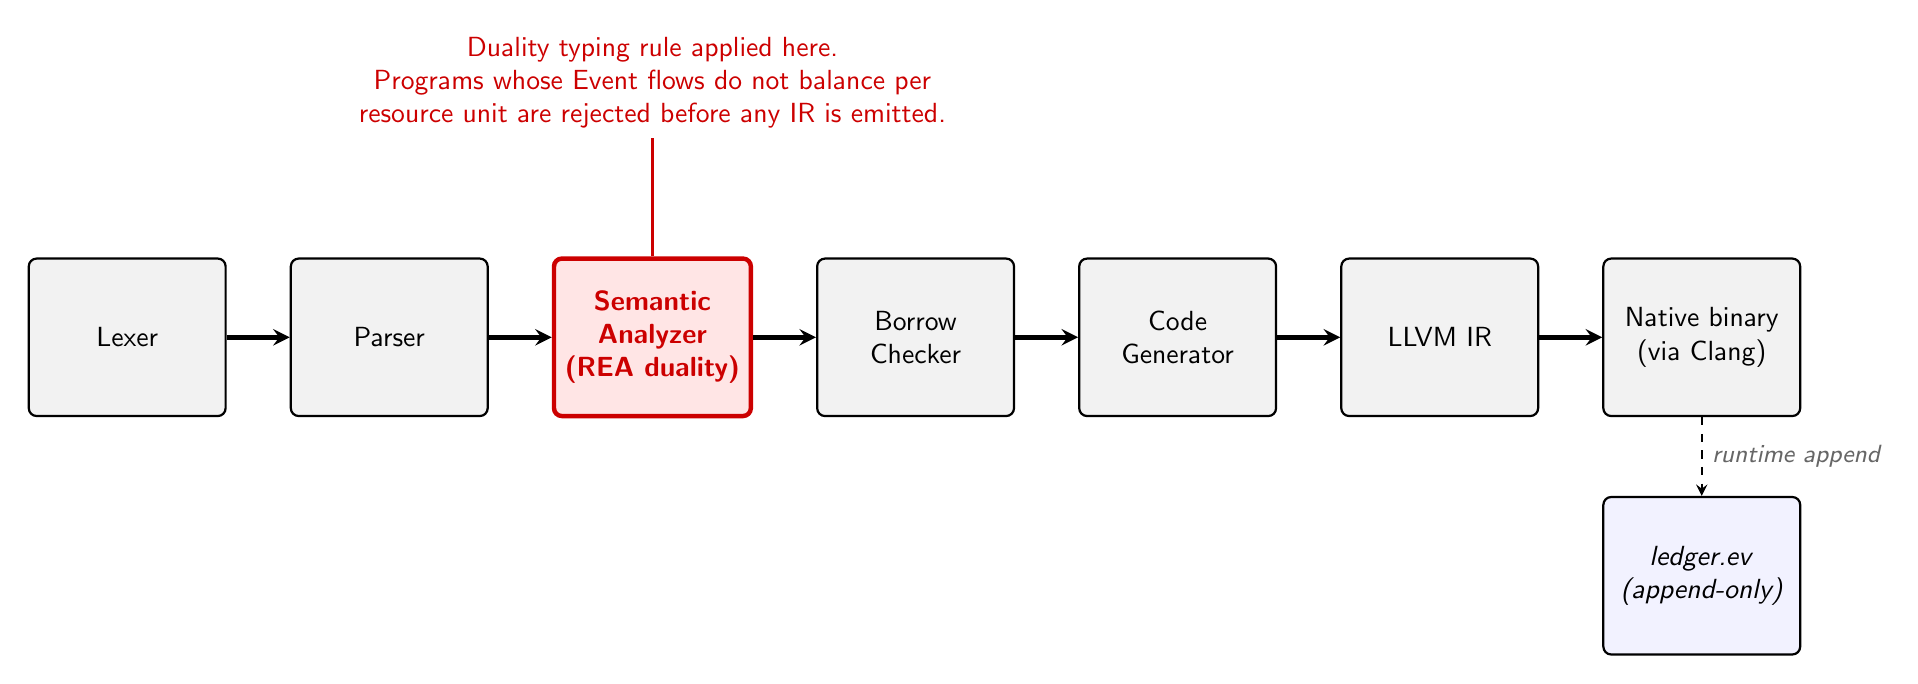
\begin{tikzpicture}[
  node distance=0.8cm,
  box/.style={draw, thick, fill=gray!10, rounded corners=1mm,
              minimum width=2.5cm, minimum height=2cm, align=center,
              font=\sffamily},
  hlbox/.style={draw, ultra thick, red!80!black, fill=red!10,
                rounded corners=1mm, minimum width=2.5cm, minimum
                height=2cm, align=center, font=\sffamily\bfseries},
  arr/.style={draw, ultra thick, ->, >=stealth}
]
\node[box] (lexer) {Lexer};
\node[box, right=of lexer] (parser) {Parser};
\node[hlbox, right=of parser] (sema) {Semantic\\Analyzer\\(REA duality)};
\node[box, right=of sema] (borrow) {Borrow\\Checker};
\node[box, right=of borrow] (codegen) {Code\\Generator};
\node[box, right=of codegen] (llvm) {LLVM IR};
\node[box, right=of llvm] (native) {Native binary\\(via Clang)};
\node[box, fill=blue!5, below=1cm of native] (ledger)
  {\textit{ledger.ev}\\\textit{(append-only)}};

\draw[arr] (lexer) -- (parser);
\draw[arr] (parser) -- (sema);
\draw[arr] (sema) -- (borrow);
\draw[arr] (borrow) -- (codegen);
\draw[arr] (codegen) -- (llvm);
\draw[arr] (llvm) -- (native);
\draw[draw, thick, dashed, ->, >=stealth] (native) -- (ledger)
  node[midway, right, font=\sffamily\itshape\small, text=gray!80!black]
  {runtime append};

\draw[draw, thick, red!80!black] (sema.north) -- ++(0, 1.5)
  node[above, text=red!80!black, font=\sffamily, align=center]
  {Duality typing rule applied here.\\
   Programs whose Event flows do not balance per\\
   resource unit are rejected before any IR is emitted.};
\end{tikzpicture}
}
\caption{The Equis compiler pipeline. Six conventional stages plus one
novel one. Programs whose Event flows do not balance are rejected at the
Semantic Analyzer before any IR is emitted.}
\label{fig:pipeline}
\end{figure}

The Equis compiler pipeline (\Cref{fig:pipeline}) consists of seven
stages: Lexer, Parser, Semantic Analyzer, Borrow Checker, Code
Generator, LLVM~IR emission, and native binary production via Clang.
The Lexer tokenizes the source with string interning for identifiers.
The Parser is a recursive-descent parser that produces an AST. The
Semantic Analyzer is the novel stage: it resolves symbols, verifies REA
duality for every event declaration, enforces role compatibility at
execute sites, and maintains the resource balance map. The Borrow
Checker performs the \textsc{Available}/\textsc{Moved} state analysis
described in \Cref{sec:design:arc}. The Code Generator traverses the
type-checked AST and emits LLVM~IR directly. Clang serves as the
assembler and linker, producing optimized native machine code from the
IR.

The Semantic Analyzer (\texttt{compiler/semantics.equis}) is the only
stage without a close analogue in a conventional compiler. All other
stages follow well-established compiler design patterns. This is
intentional: Equis's contribution is a domain-semantic addition to an
otherwise conventional pipeline, following the principle established by
\citet{leroy_formal_2009} that a formally structured pipeline with a novel
verified stage is more trustworthy than a monolithic verifier. The
compiler is self-hosted: it is written in Equis and compiled by itself.

\subsection{The self-hosting bootstrap}

\begin{figure}[ht]
\centering
\resizebox{\textwidth}{!}{
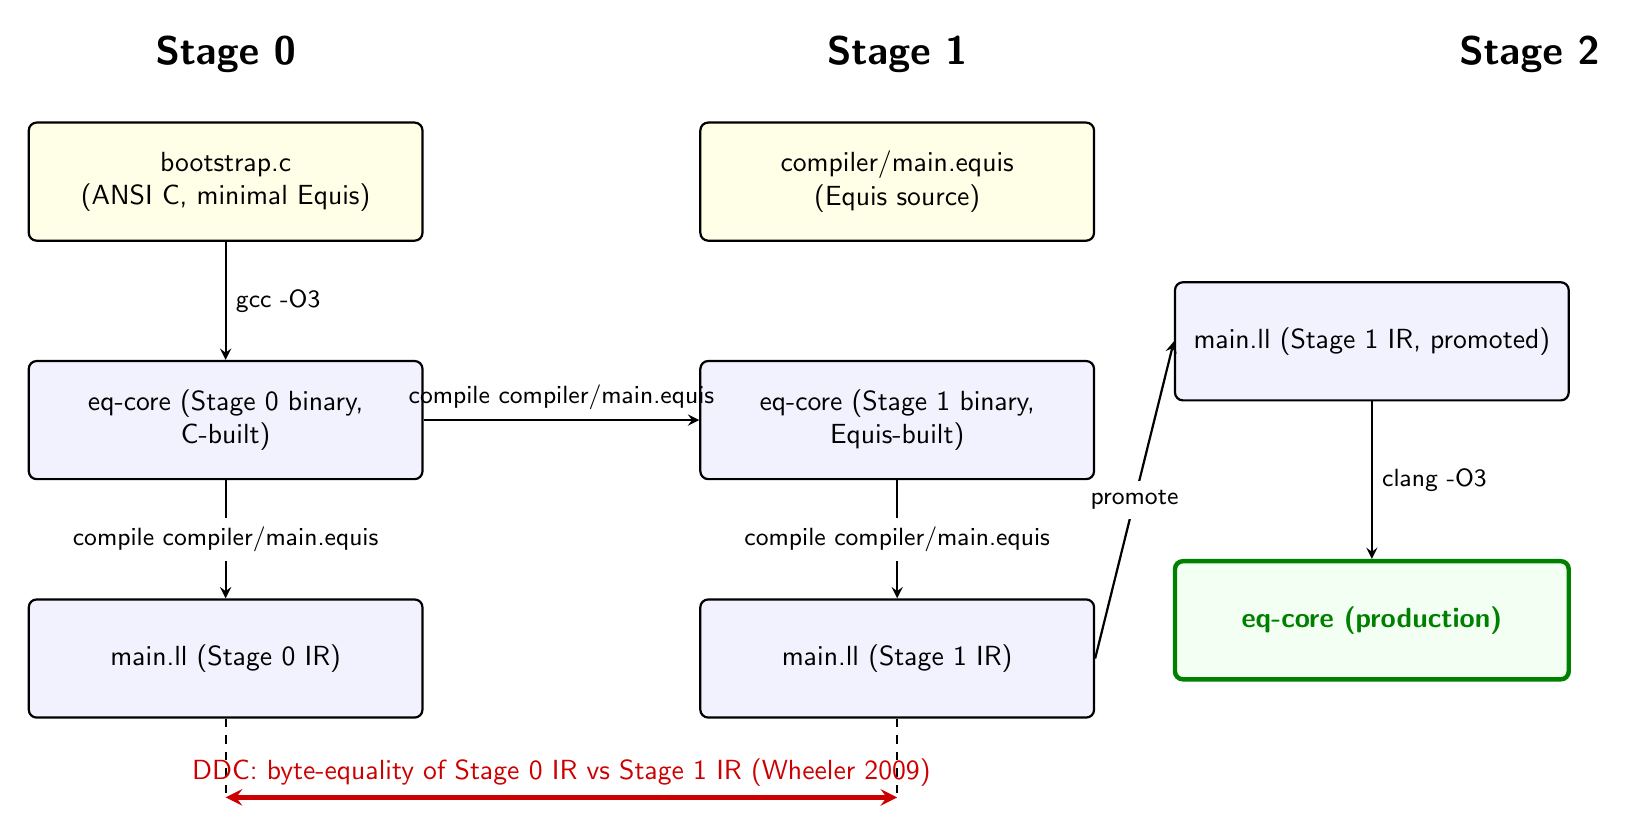
\begin{tikzpicture}[
  node distance=1cm and 2cm,
  box/.style={draw, thick, fill=blue!5, rounded corners=1mm,
              minimum width=5cm, minimum height=1.5cm, align=center,
              font=\sffamily},
  ybox/.style={draw, thick, fill=yellow!10, rounded corners=1mm,
               minimum width=5cm, minimum height=1.5cm, align=center,
               font=\sffamily},
  gbox/.style={draw, ultra thick, green!50!black, fill=green!5,
               rounded corners=1mm, minimum width=5cm, minimum
               height=1.5cm, align=center, font=\sffamily\bfseries},
  arr/.style={draw, thick, ->, >=stealth}
]
\node[font=\sffamily\Large\bfseries] (s0) {Stage 0};
\node[font=\sffamily\Large\bfseries, right=6.5cm of s0] (s1) {Stage 1};
\node[font=\sffamily\Large\bfseries, right=6cm of s1] (s2) {Stage 2};

\node[ybox, below=0.5cm of s0] (b0)
  {bootstrap.c\\(ANSI C, minimal Equis)};
\node[ybox, below=0.5cm of s1] (b1)
  {compiler/main.equis\\(Equis source)};

\node[box, below=1.5cm of b0] (e0)
  {eq-core (Stage 0 binary,\\C-built)};
\node[box, below=1.5cm of b1] (e1)
  {eq-core (Stage 1 binary,\\Equis-built)};

\node[box, below=1.5cm of e0] (i0) {main.ll (Stage 0 IR)};
\node[box, below=1.5cm of e1] (i1) {main.ll (Stage 1 IR)};

\node[box, right=1cm of e1, yshift=1cm] (i2)
  {main.ll (Stage 1 IR, promoted)};
\node[gbox, below=2cm of i2] (prod) {eq-core (production)};

\draw[arr] (b0) -- (e0)
  node[midway, right, font=\sffamily\small] {gcc -O3};
\draw[arr] (e0) -- (i0)
  node[midway, fill=white, font=\sffamily\small]
  {compile compiler/main.equis};
\draw[arr] (e0) -- (e1)
  node[midway, above, font=\sffamily\small]
  {compile compiler/main.equis};
\draw[arr] (e1) -- (i1)
  node[midway, fill=white, font=\sffamily\small]
  {compile compiler/main.equis};

\draw[arr] (i1.east) -- (i2.west)
  node[midway, fill=white, font=\sffamily\small] {promote};
\draw[arr] (i2) -- (prod)
  node[midway, right, font=\sffamily\small] {clang -O3};

\draw[draw, thick, dashed] (i0.south) -- ++(0,-1) coordinate (c0);
\draw[draw, thick, dashed] (i1.south) -- ++(0,-1) coordinate (c1);
\draw[draw, ultra thick, red!80!black, <->, >=stealth] (c0) -- (c1)
  node[midway, above, text=red!80!black, font=\sffamily]
  {DDC: byte-equality of Stage 0 IR vs Stage 1 IR (Wheeler 2009)};
\end{tikzpicture}
}
\caption{Three-stage bootstrap and Diverse Double Compilation
verification. If the IR produced by the C-built Stage 0 compiler
matches the IR produced by Stage 1 byte for byte, neither can contain a
backdoor that is absent from either source program.}
\label{fig:bootstrap}
\end{figure}

The bootstrap process follows three stages, documented in
\texttt{bootstrap.ps1} and \texttt{Makefile} (\Cref{fig:bootstrap}).

\paragraph{Stage 0.} An ANSI~C program (\texttt{bootstrap.c}) implements
a minimal subset of the Equis language, sufficient to parse and compile
the Equis-written compiler source, but not a full implementation. This
stage is compiled once: \texttt{gcc -O3 bootstrap.c -o eq-core}.

\paragraph{Stage 1.} The Stage 0 binary compiles the Equis compiler
source to LLVM~IR:
\texttt{eq-core -I std compiler/main.equis > compiler/main.ll}. The
resulting IR is a complete representation of the Equis compiler, as
produced by the minimal C implementation.

\paragraph{Stage 2.} Clang compiles the LLVM~IR to a production native
binary: \texttt{clang -O3 compiler/main.ll runtime.c -o eq-core}. This
binary replaces the Stage 0 binary and is thereafter the authoritative
Equis compiler.

\citet{thompson_reflections_1984} showed in ``Reflections on Trusting
Trust'' that a self-hosting compiler can embed invisible backdoors: a
malicious compiler could inject code into programs it compiles without
any evidence in the source. Equis addresses this through Diverse Double
Compilation (DDC), described by \citet{wheeler_fully_2009}: the Stage 0
(C-compiled) and Stage 1 (Equis-compiled) outputs are compared at the
LLVM~IR level. If the two independently produced compilers emit
identical IR for the same input, neither can contain a backdoor that is
absent from the source, since a backdoor would require a discrepancy.
The DDC verification pass is part of the build system.

\subsection{LLVM~IR code generation}

The code generator emits LLVM~IR instructions directly, without using
the LLVM C API. Fixed-point addition and subtraction map to
\texttt{add i64} and \texttt{sub i64}:

\begin{llvmcode}
; decimal addition: a + b
%result = add i64 %a, %b
\end{llvmcode}

Fixed-point multiplication calls \texttt{fixed\_mul}, whose body
contains a \texttt{mul i64} followed by \texttt{sdiv i64 1000000}. No
\texttt{fadd}, \texttt{fmul}, \texttt{fdiv}, or any other floating-point
instruction appears in financial code paths. The code generator verifies
this invariant during emission.

A representative LLVM~IR fragment for a \texttt{PurchaseOrder} event
body demonstrates that the compiled output is integer-only:

\begin{llvmcode}
define void @equis_event_PurchaseOrder(i64 %buyer_id,
                                       i64 %seller_id) {
entry:
  ; transfer 12 StockItem: out from Seller, in to Buyer
  %qty    = add i64 0, 12000000          ; 12 units * 1000000
  ; transfer 600 USD: out from Buyer, in to Seller
  %amount = add i64 0, 600000000         ; 600 USD * 1000000
  ; ledger append (append-only, no delete)
  call void @ledger_append_event(i64 %qty, i64 %amount)
  ret void
}
\end{llvmcode}

\subsection{ARC emission}

The ownership analysis pass inserts \texttt{sys\_retain} and
\texttt{sys\_release} calls at ownership transfer points. For
arena-allocated objects, the pass instead records the allocation in the
current arena and emits \texttt{arena\_free\_all} at scope exit. Cyclic
references within event graphs are detected during the Semantic
Analysis phase (not the borrow checker), because a cycle in the
resource flow graph would represent a circular economic dependency,
that is, an event whose execution requires itself.

\citet{ullrich_counting_2021} showed that the key optimization for ARC in
functional programming is deferring decrements until after the
operation that needs the value, allowing the runtime to reuse the
storage in place. Equis applies an analogous approach in its imperative
context: the code generator defers release calls to the end of the
smallest enclosing block rather than emitting them immediately after
the last use.

\subsection{Standard library}

The standard library comprises 20 modules (\Cref{tab:stdlib}).

\begin{table}[ht]
\caption{Standard library modules.}
\label{tab:stdlib}
\centering
\small
\begin{tabular}{@{}ll@{}}
\toprule
Module & Description \\
\midrule
\texttt{std.sys}         & Memory, syscall bindings, runtime primitives \\
\texttt{std.string}      & String manipulation and formatting \\
\texttt{std.collections} & Dynamic arrays and hash maps \\
\texttt{std.arena}       & Linear bump-pointer arena allocator \\
\texttt{std.fixed}       & Fixed-point arithmetic (the \texttt{decimal} implementation) \\
\texttt{std.ledger}      & Append-only \texttt{ledger.ev} API \\
\texttt{std.accounting}  & Trial balance, income statement, balance sheet \\
\texttt{std.compliance}  & ESG and regulatory constraint checks \\
\texttt{std.db}          & PostgreSQL connector (parameterized queries only) \\
\texttt{std.json}        & JSON serialization and deserialization \\
\texttt{std.http}        & HTTP server \\
\texttt{std.chan}        & Thread-safe typed channels \\
\texttt{std.fiber}       & Preemptive fiber scheduler \\
\texttt{std.ffi}         & Foreign function interface to C \\
\texttt{std.net}         & Socket networking \\
\texttt{std.rpc}         & Remote procedure calls \\
\texttt{std.intern}      & String interning \\
\texttt{std.dual\_net}   & Distributed duality verification \\
\bottomrule
\end{tabular}
\end{table}

The \texttt{std.db} module accepts only parameterized queries; string
interpolation into SQL is a compile-time error, preventing SQL injection
at the language level. The \texttt{std.ledger} module exposes only
append operations; no update or delete path exists.

%% ---------------------------------------------------------------------------
\section{Formal Semantics}\label{sec:semantics}
%% ---------------------------------------------------------------------------

\subsection{Syntax and typing environments}

The abstract syntax for REA declarations is:
\[
\begin{array}{rcl}
\mathit{decl} & ::= & \texttt{Resource } \mathit{id}\ \{ \texttt{unit:}\ \mathit{str};\ \texttt{decimals:}\ \mathit{int}; \} \\
              & \mid & \texttt{Agent } \mathit{id} \texttt{ roles } \{ \mathit{str}^{*} \}\ \{ \mathit{field}^{*} \} \\
              & \mid & \texttt{Commitment } \mathit{id} \texttt{ evaluated\_by } \mathit{id}\ \{ \mathit{flow} \} \\
              & \mid & \texttt{Event } \mathit{id} \texttt{ fulfills } \mathit{id} \texttt{ roles } \{ \mathit{str}^{*} \} \\
              &      & \qquad \{ \mathit{logic};\ \mathit{flow} \} \\[0.5ex]
\mathit{flow} & ::= & \texttt{flow }\{ \mathit{flowdir}^{*} \} \\
\mathit{flowdir} & ::= & \texttt{in } \mathit{int}\ \mathit{id} \texttt{ from } \mathit{id} \texttt{ to } \mathit{id}; \\
                 & \mid & \texttt{out } \mathit{int}\ \mathit{id} \texttt{ from } \mathit{id} \texttt{ to } \mathit{id};
\end{array}
\]
A typing environment $\Gamma$ maps each identifier to a triple
$(\mathrm{Type},\ \mathrm{RoleSet},\ \mathrm{BalanceEntry})$.
$\mathrm{Type}$ ranges over $\mathrm{ResourceType}$,
$\mathrm{AgentType}$, $\mathrm{EventType}$, and
$\mathrm{CommitmentType}$. $\mathrm{RoleSet}$ is a set of role strings.
$\mathrm{BalanceEntry}$ is a rational number representing the net
resource flow attributed to the identifier in the current event
context.

\subsection{The duality typing rule}

The full multi-leg duality rule is:
\[
\dfrac{
  \begin{array}{c}
    \forall i:\ \Gamma \vdash r_i : \mathrm{ResourceType}(unit_i) \\
    I = \{\, i \mid \mathit{direction}_i = \texttt{in}\,\} \quad
    D = \{\, j \mid \mathit{direction}_j = \texttt{out}\,\} \\
    \forall i,j \in I \cup D:\ unit_i = unit_j \quad \text{(unit homogeneity)} \\
    \sum_{i \in I} \mathit{amount}_i = \sum_{j \in D} \mathit{amount}_j \quad \text{(balance)} \\
    \forall i:\ \mathit{amount}_i > 0 \quad \text{(positive flows)}
  \end{array}
}{
  \Gamma \vdash \texttt{Event } id\ \{\, \texttt{flow }\{ \mathit{flowdir}_1, \dots, \mathit{flowdir}_n \}\,\} : \mathrm{BalancedEvent}(unit)
}
\]

\begin{theorem}[Duality, multi-leg form]\label{thm:duality-full}
If $\Gamma \vdash e : \mathrm{BalancedEvent}(u)$, then for all states
$\sigma$ satisfying $\Gamma$, executing $e$ in $\sigma$ produces
$\sigma'$ such that
\[
\sum_{a \in \mathrm{Agents}} \mathrm{holdings}(a, u, \sigma') =
\sum_{a \in \mathrm{Agents}} \mathrm{holdings}(a, u, \sigma).
\]
\end{theorem}

\begin{proof}
By structural induction on the derivation tree. The base case is a
single inflow--outflow pair: executing the event transfers
$\mathit{amount}$ units of $u$ from one agent's holdings to another,
preserving the total. For the inductive case, a composed event with
flows $F_1,\dots,F_n$ has total inflows equal to total outflows by the
balance premise. The execution of each flow preserves the invariant by
the inductive hypothesis applied to each sub-transfer. The sum of
balanced sub-transfers is balanced.
\end{proof}

The balance check is $O(n)$ in the number of flow directives and is
performed during the Semantic Analysis pass, before code generation. It
introduces no runtime overhead.

\subsection{ARC soundness}

The borrow checker maintains a map from resource identifier to state in
$\{\textsc{Available},\ \textsc{Moved}\}$. The transitions are:
\begin{itemize}\setlength{\itemsep}{0pt}
  \item On declaration: state $\to$ \textsc{Available}.
  \item On function call with ownership transfer: state $\to$ \textsc{Moved}.
  \item On read of a \textsc{Moved} identifier: type error (use-after-move).
\end{itemize}

\begin{theorem}[ARC Soundness]\label{thm:arc}
If the borrow checker accepts a program $P$, then no resource value in
$P$ is accessed after its retain count reaches zero.
\end{theorem}

\begin{proofsketch}
The borrow checker's \textsc{Available}/\textsc{Moved} analysis is a
conservative abstraction of the retain count: a resource is
\textsc{Moved} (retain count zero) whenever it has been passed to a
consuming call. Any read of a \textsc{Moved} resource is rejected.
Since the borrow checker accepts only programs where no read follows a
move, no read occurs after retain count zero. \qed
\end{proofsketch}

Cyclic references are prohibited by the type system. A cycle in the
resource flow graph is detected during Semantic Analysis as a duality
violation, since a resource cannot simultaneously flow into and out of
the same event without external input. This makes the ARC
implementation cycle-free, eliminating the one classical failure mode
of reference counting.

\subsection{Fixed-point arithmetic precision}

\begin{proposition}\label{prop:fp}
For any two \texttt{decimal} values $a, b$ with $|a|, |b| < 2^{57}$, the
result of $\texttt{fixed\_add}(a,b)$ equals the mathematical value
$a+b$, and the result of $\texttt{fixed\_mul}(a,b)$ differs from the
mathematical value $a \times b$ by at most $10^{-6}$.
\end{proposition}

\begin{proof}
Addition: both operands and the result are exact 64-bit integers; no
rounding occurs. Multiplication: the result is
$\lfloor (a \times b)/10^{6}\rfloor$ with banker's rounding applied to
the remainder. The error is $|r/10^{6}| \le 0.5 \times 10^{-6}$.
\end{proof}

This bound is tighter than any IEEE 754 double-precision accumulation
scenario by eight orders of magnitude for single-operation errors, and
the errors do not compound across additions (only across
multiplications).

\subsection{RBAC type safety}

Roles are strings assigned to agents and required by events. The
compiler maintains a role compatibility relation: an event execution is
type-safe if and only if the executing agent's role set intersects with
the event's required role set. The check is performed at
\texttt{execute} callsites during Semantic Analysis.

\begin{proposition}[RBAC Soundness]\label{prop:rbac}
If the semantic analyzer accepts a program $P$, then every event
execution in $P$ is performed by an agent whose declared roles satisfy
the event's role requirement.
\end{proposition}

%% ---------------------------------------------------------------------------
\section{Evaluation}\label{sec:eval}
%% ---------------------------------------------------------------------------

\subsection{Supply chain settlement scenario}

To demonstrate the language's correctness guarantees in a realistic
context, consider a three-party supply chain settlement: a
\textbf{Supplier} delivers goods to a \textbf{Buyer}, with a
\textbf{Clearinghouse} facilitating payment. The scenario involves a
commitment, an event fulfilling it, and a partial reversal.

\paragraph{Resource and agent declarations.}

\begin{equiscode}
Resource USD       { unit: "USD"; decimals: 2; }
Resource StockItem { unit: "PCS"; }

Agent Buyer         roles { "CONSUMER" }     { id: "B1";  ... }
Agent Supplier      roles { "VENDOR" }       { id: "S1";  ... }
Agent Clearinghouse roles { "INTERMEDIARY" } { id: "CH1"; ... }
\end{equiscode}

\paragraph{Procurement commitment.}

\begin{equiscode}
Commitment ProcurementOrder evaluated_by MarketRate {
    flow {
        out 500 StockItem from Supplier to Buyer;
        in  10000 USD from Buyer to Supplier;
    }
}
\end{equiscode}

\paragraph{Fulfilling event.}

\begin{equiscode}
Event SupplyDelivery fulfills ProcurementOrder roles { "CONSUMER" } {
    logic {
        assert(1 > 0);
    }
    flow {
        in  500 StockItem from Supplier to Buyer;
        out 10000 USD from Buyer to Clearinghouse;
        in  10000 USD from Clearinghouse to Supplier;
    }
}

execute SupplyDelivery { sig: Buyer; timestamp: "1711449600" };
\end{equiscode}

\paragraph{Partial reversal.}

\begin{equiscode}
reverse SupplyDelivery { reason: "50 units damaged in transit" };
\end{equiscode}

The reversal appends a compensating event to \texttt{ledger.ev}. The
original delivery record is never deleted. The \texttt{std.accounting}
module, when queried for the net position of \texttt{StockItem}, sums
both entries and returns 450 units net delivered.

\paragraph{Deliberate error: unbalanced event.}

\begin{equiscode}
Event BrokenDelivery fulfills ProcurementOrder roles { "CONSUMER" } {
    flow {
        in  500 StockItem from Supplier to Buyer;
        // outflow omitted, programmer forgot the payment leg
    }
}
\end{equiscode}

Compilation output:

\begin{plaincode}
error: REA Duality Violation: Economic Event must have reciprocal
       flows (In and Out).
\end{plaincode}

The compiler rejects this program. An equivalent Python implementation
would accept this function without error; the missing payment would
manifest as a runtime ledger imbalance, detectable only by
reconciliation.

\subsection{Correctness evaluation}

The project includes a test suite that covers duality enforcement, ARC
correctness, RBAC enforcement, and fixed-point arithmetic. The test
methodology for duality enforcement injects deliberately malformed
programs, including events with missing outflows, events with
mismatched amounts, and events with no flow block, and verifies that
each is rejected at compile time. Role injection tests verify that
\texttt{execute} callsites with insufficient roles are rejected.
Fixed-point tests verify arithmetic identities and banker's rounding
behavior.

\subsection{Runtime throughput}

Throughput is measured by the benchmark in
\path{examples/benchmarks/speed_test.equis}, which performs one million
iterations of \texttt{total = total + 1.25} in fixed-point i64
representation. The Equis compiler emits explicit \texttt{sys\_retain}
and \texttt{sys\_release} calls at every variable read inside the loop,
so the inner loop measures fixed-point addition together with ARC
bookkeeping rather than addition in isolation. Each row in
\Cref{tab:throughput} is the median of five runs.

\begin{table}[ht]
\caption{Runtime throughput benchmarks.}
\label{tab:throughput}
\centering
\small
\begin{tabular}{@{}lr@{}}
\toprule
Variant & Median (ms) \\
\midrule
Equis fixed-point i64 ($\times 10^{6}$), \texttt{clang -O0} & 1020.78 \\
Equis fixed-point i64 ($\times 10^{6}$), \texttt{clang -O1} & 1011.55 \\
Equis fixed-point i64 ($\times 10^{6}$), \texttt{clang -O2} & 1015.97 \\
Equis fixed-point i64 ($\times 10^{6}$), \texttt{clang -O3} & 1022.38 \\
Python \texttt{decimal.Decimal}                              &   62.50 \\
Python \texttt{int} fixed-point ($\times 10^{6}$)            &   35.83 \\
Python \texttt{float} (IEEE 754 double)                       &   28.96 \\
C \texttt{int64\_t} fixed-point, \texttt{gcc -O2} with sink  &    0.20 \\
\bottomrule
\end{tabular}
\end{table}

Two facts are worth flagging. First, the Equis numbers are essentially
identical across \texttt{-O0}, \texttt{-O1}, \texttt{-O2}, and
\texttt{-O3}, which confirms that the ARC retain and release calls
survive LLVM's dead-code analysis as externally-visible side effects on
the runtime reference-count state. The optimizer cannot fold the loop
away. Second, the Equis runtime is roughly 16 times slower than
\texttt{decimal.Decimal} and four orders of magnitude slower than raw
C integer arithmetic on this microbenchmark. That cost buys
compile-time duality enforcement, role-checked event execution, and the
borrow checker; none of those properties is available in any other
entry of the table.

In production accounting workloads the picture changes. Each event
commit involves at least one ledger \texttt{fsync}, which on the same
hardware costs roughly 100 microseconds for a small JSON record on a
consumer NVMe SSD. The per-iteration ARC overhead measured above is
approximately one microsecond, two orders of magnitude below the
per-event I/O floor. ARC is therefore amortized below the noise of
disk I/O for any code path that actually touches the ledger, which is
the only code path where duality matters.

ARC additionally provides deterministic memory reclamation with no
stop-the-world pauses. Worst-case allocation latency is bounded by the
size of the single largest individual allocation, not by the size of
the live heap, which is the property settlement systems require for
tail latency under load.

\subsection{Compile-time cost of duality checking}

The duality check is $O(n)$ in the number of flow directives within an
event and is run once per event declaration during the Semantic
Analysis pass. \Cref{tab:compile} reports compile times for synthetic
programs containing $N$ event declarations, each with two flow
directives. Compile time is measured as the wall clock of
\texttt{eq-core -I . events\_N.equis > /dev/null} on Ubuntu under WSL2.

\begin{table}[ht]
\caption{Compile-time cost of duality checking.}
\label{tab:compile}
\centering
\small
\begin{tabular}{@{}rr@{}}
\toprule
$N$ events & Median compile time (s) \\
\midrule
   10 & 0.087 \\
  100 & 0.165 \\
 1000 & 2.616 \\
\bottomrule
\end{tabular}
\end{table}

Up to roughly one hundred event declarations per source file, the
duality check and surrounding semantic analysis are dominated by
parsing and IR emission. Beyond that point compile time grows
superlinearly as IR string size dominates. For typical accounting
modules with tens to a low hundred of event types per source file,
compilation finishes in under 200~ms.

\subsection{Benchmark methodology}

All benchmarks were run on a 12th-generation Intel Core i5-1235U with
15.7~GB RAM. The host OS is Windows 11 Home Single Language 10.0.26200;
WSL2 runs Ubuntu with kernel 6.6.87.2-microsoft-standard-WSL2. The
toolchain consists of clang 22.1.2, gcc 16.0.1 (MinGW-W64 ucrt), and
Python 3.12.5. The Equis runtime corresponds to v0.1.0 stage~2. Each
benchmark program was run five times after a single warm-up run; the
warm-up run was discarded. Wall-clock time was measured with
\texttt{System.Diagnostics.Stopwatch} for Windows binaries, with
\texttt{time.perf\_counter} for Python, and with \texttt{bash time}
for compile-time measurements. Raw per-run numbers are recorded in
\texttt{bench\_results.txt} alongside the paper source for independent
verification.

The performance trade-off baked into Equis is deliberate. Exact
arithmetic with deterministic error bounds and compile-time enforcement
of accounting invariants is worth more in financial contexts than
maximally fast approximate arithmetic. The numbers above are presented
to characterize the cost, not to argue that it is zero.

%% ---------------------------------------------------------------------------
\section{Related Work}\label{sec:related}
%% ---------------------------------------------------------------------------

\subsection{REA-based systems}

\citet{mccarthy_rea_1982} is the founding reference. It introduced the
three-primitive model and the duality axiom, but it described a
database schema design, not a programming language. The ontological
analyses of \citet{geerts_ontological_1999,geerts_ontological_2002}
established first-order logical foundations for REA and proved that
duality is a theorem in the ontology, not merely a convention.
\citet{geerts_policy-level_2006} added authorization specifications. All of
this work operates at the modeling layer; none of it produces machine
code.

The REA-DSL of \citet{sonnenberg_rea-dsl_2011} is the closest prior work
to a language-level implementation. It provides a notation for
specifying REA models and validates them against the ontological
constraints. It is, however, a modeling language that produces model
artifacts, not a compiled systems language that produces executable
financial infrastructure.

\citet{dunn_rea_1997} surveyed the intellectual heritage of REA and its
prospects for extension. \citet{ibanez_rea_2020} argued that REA,
triple-entry accounting, and blockchain ledgers represent convergent
approaches to shared ledger systems, but their work is at the
architectural level, not the language level. \citet{oleary_mitigating_2025}
extended REA with location and hierarchy concepts, demonstrating the
model's continued vitality in the research community, while remaining
at the database/knowledge-representation layer.

\subsection{Formally verified compilers}

\citet{leroy_formal_2009} is the landmark result in formally verified
compilation: a complete C compiler proved correct in Coq, with a
theorem stating that the compiled code's behavior matches the source
program's semantics. CompCert does not encode domain semantics; it
verifies that compilation preserves general program behavior.
\citet{klein_machine-checked_2006} verified a JVM-like language and virtual
machine in Isabelle/HOL, establishing the methodology for
machine-checked compiler correctness.

Equis's contribution is orthogonal to these. The Equis compiler is not
formally verified in the CompCert sense; its correctness rests on the
DDC bootstrap verification and conventional testing. The novelty is the
domain-semantic duality type rule, not compiler correctness proofs.
Machine verification of the duality theorem in Coq is future work.

\subsection{Financial DSLs and contract languages}

\citet{andersen_compositional_2006} developed a compositional denotational
semantics for financial contracts, providing a formal basis for
specifying, analyzing, and pricing contracts.
\citet{henglein_formally_2020} extended this with static analysis and
mechanized verification. These are specification languages for
financial instruments, not systems languages for building financial
infrastructure. They describe what a contract means; they do not
compile to code that settles the contract.

Marlowe, developed for the Cardano blockchain, is a similar financial
contract DSL. It is deliberately limited in expressiveness to make
formal analysis tractable. It targets smart contract execution
environments, not general systems programming. Neither Marlowe nor the
Andersen/Henglein line of work produces an executable systems language
with REA primitives.

\subsection{Memory-safe systems languages}

Rust provides ownership types and borrow checking that guarantee memory
safety and data-race freedom at compile time. The grounded conceptual
model of \citet{crichton_grounded_2023} formalizes Rust's ownership
system using place-capability graphs. Rust's type system is
domain-agnostic: it does not know what a financial transaction is and
cannot enforce duality. Equis borrows the move-semantics concept from
Rust and applies it in a financial-domain context, using a simpler
resource-state map (\textsc{Available}/\textsc{Moved}) rather than the
full place-capability graph.

\citet{ullrich_counting_2021} established that ARC can be made
competitive with tracing GC through careful optimization of
retain/release placement. Swift's ARC implementation
\citep{ungar_dynamic_2017} demonstrates the same principle in a
production systems language. Equis applies ARC in a domain where
deterministic reclamation is an operational requirement, not merely a
performance preference.

\citet{bernardy_linear_2017} introduced practical linear types into a
polymorphic functional language, tracking that resources are used
exactly once. Linear types and accounting duality address related but
distinct concerns: linear types prevent resource duplication and loss;
duality requires that resource transfer be balanced across agents.
Equis's move semantics are analogous to linear types in their
prevention of aliasing, but the duality rule goes further by requiring
flow balance.

\citet{rastogi_wys_2018} shows that domain-specific security properties
(secure multi-party computation) can be embedded in a language
extension with formal verification. This is the closest methodological
analogue to Equis: a language-level invariant for a security-critical
domain, enforced by the compiler.

%% ---------------------------------------------------------------------------
\section{Discussion}\label{sec:discussion}
%% ---------------------------------------------------------------------------

\subsection{Limitations}

The duality checker currently handles events where all flows are in
the same unit of measure. Multi-currency events, where the buyer pays
in EUR and the seller receives in USD, require explicit currency
conversion events using a declared Valuator. Automatic FX rate
application is not supported. This is a deliberate design choice:
currency conversion is itself an economic event with its own duality
requirements, and making it explicit keeps the type system sound.
Automatic conversion would require embedding an FX rate oracle into
the type checker, which would couple language semantics to external
data.

The Duality Theorem is proved by hand. Machine verification in Coq or
Isabelle/HOL, following the methodology of \citet{klein_machine-checked_2006},
is planned but not yet complete. The hand proof is straightforward by
induction on the derivation tree, as shown in
\Cref{thm:duality-full}, but a mechanized proof would provide stronger
assurance and enable formal reasoning about extensions.

The standard library currently provides a PostgreSQL connector only.
Other database backends (MySQL, SQLite, Oracle) would require FFI
bindings or native driver implementations. The FFI module
(\texttt{std.ffi}) makes these possible but they are not yet part of
the standard library.

The language is at version 0.1.0. The semantics are stable, but some
standard library modules (particularly \texttt{std.rpc} and
\texttt{std.dual\_net}) are marked experimental and their APIs may
change.

\subsection{Future work}

The most immediate extension is multi-currency support: a
units-of-measure type system for \texttt{decimal} values that tracks
the currency as part of the type and requires explicit FX conversion
events at points where currencies are mixed. This would make the type
checker currency-aware while preserving the current duality rule.

Machine verification of the formal semantics in Coq is the
highest-priority correctness improvement. The operational semantics
are specified informally in \Cref{sec:semantics}; a Coq formalization
would follow the structure of the Jinja work
\citep{klein_machine-checked_2006} and provide a mechanized proof of the
Duality Theorem.

Distributed settlement, where events are committed across multiple
nodes under potential network partitions, raises consistency questions
not addressed by the current single-node ledger design. A formal
consistency model for distributed Equis deployments, drawing on the
literature on distributed ledger systems, is planned.

The relationship between Equis and smart contract languages (Marlowe,
Solidity) deserves a formal expressiveness comparison. Both address
financial correctness, but from different starting points: smart
contracts begin with a distributed execution model and add financial
concepts; Equis begins with a financial type system and adds systems
programming capabilities. A formal comparison of what each can and
cannot express would clarify the design space.

Dependent types could enable higher-order invariants: for example, a
type-level proof that the total inventory across a full supply chain
is conserved across all shipment events. The current type system
enforces duality per-event; dependent types could extend this to
multi-event sequences.

%% ---------------------------------------------------------------------------
\section{Conclusion}\label{sec:conclusion}
%% ---------------------------------------------------------------------------

The financial software industry has spent four decades applying
McCarthy's REA framework at the modeling layer, in database schemas,
business process diagrams, and markup languages. The same framework
has not, until now, been applied at the language layer, where it could
actually prevent the errors it describes.

Equis demonstrates that REA primitives can be first-class syntax
constructs in a compiled systems language, that accounting duality
can be expressed as a typing rule and proved sound, and that a
self-hosting compiler can enforce these properties with zero runtime
overhead. The language is practical: it compiles to native machine
code via LLVM, supports PostgreSQL, HTTP, concurrent fibers, and RPC,
and ships with a 20-module standard library covering the full range
of financial application requirements.

The broader implication is methodological. Equis is an instance of
the principle that domain-critical invariants belong in language
definitions, not in application frameworks. The same principle could
be applied in other safety-critical domains: medical device software
subject to FDA 21 CFR Part 11 audit requirements, aviation software
under DO-178C, nuclear instrumentation. In each case, the invariants
are well-understood, formally specifiable, and currently enforced
only by convention. A language whose type system embodies those
invariants would make an entire class of domain-specific bugs
impossible, at compile time, for the cost of a domain-aware type
checker.

Forty years of REA theory have produced a rigorous foundation for this
approach. Equis is an attempt to make that foundation executable.

%% ---------------------------------------------------------------------------
%%  Bibliography
%% ---------------------------------------------------------------------------
\printbibliography

\end{document}
